\title{''Raplh Spaccatutto''}

\author{Enrico Cornacchia \\ Giulia Golesano \\ Giovanni Rinchiuso \\ Nikolai Zanni}
\date{10 giugno 2024}

\begin{document}

\maketitle

\tableofcontents

\chapter{Analisi}

\section{Requisiti}

Il progetto, a noi commissionato dall'università di Bologna, si pone l'obbiettivo di ricreare un videogioco basato sul classico e celebre arcade Ralph Spaccatutto, che rientra nella categoria dei giochi platformer, ossia dei giochi in cui la meccanica di gioco implica l'attraversamento di uno o piu livelli, ognuno dei quali composto da piattaforme solitamente situate su più piani.

\subsection{Requisiti funzionali}

\begin{itemize}


	//SPIEGA MEGLIO COME FUNZIONA IL GIOCO
	\item Felix, il protagonista del gioco, avrà l'obiettivo di aggiustare tutte le finestra del condominio rotte dall'antagonista Ralph. 
	\item Per arrivare a tale scopo, potrà muoversi a destra e a sinistra lungo ogni piattaforma, che rappresenta un piano del condominio, per poi salire o scendere agli altri piani.
	\item Una complicazione che incontrerà il protagonista sono i mattoni che durante tutta la partita Ralph lancerà dalla sua piattaforma in cima al condominio, che Felix quindi dovrà schivare per non perdere le sue 3 vite a dispozione.
	\item Degli aiuti che potrà ottenere sono invece i power ups che gli potranno garantire invincibilità per qualche secondo.
	\item I nostri requisiti funzionali prevedono, oltre al corretto funziamento del gioco, un menù iniziale da cui selezionare l'avvio, la pausa o l'arresto del gioco, tramite appositi tasti e la gestione delle condizioni di vittoria e sconfitta.
	LIVELLI ??
\end{itemize}


\subsubsection{Requisiti non funzionali}
\begin{itemize}
	\item Ci poniamo l'obiettivo di fornire un'esperienza di gioco il più fluida possibile, restando sempre fedeli alla versione originale nonostante le nostre rivisitazioni.
\end{itemize}

\section{Analisi e modelli del dominio}
//AGGIUNGERE SCALE
La schermata di gioco è composta da una facciata di condominio, simile ad una griglia, in cui si trovano, in base alla difficoltà del livello, un numero variabile di file di finestre, per ognuno dei piani del condominio.
Come anticipatamente spiegato, il player Felix dovrà aggiustare tutte le finestre schivando i mattoni lanciati da Ralph, per vincere la partita.
Per farlo, dovrà fermarsi, davanti alla finestra che desidera aggiustare, e tenere premuto il BACKSPACE per 1.5 secondi. 
Per muoversi tra i piani avrà a disposizione le 4 direzioni UP, DOWN, LEFT e RIGHT, ognuna svolta dall'apposita freccina della tastiera. 
Felix avrà un numero limitato di vite, che di default sarà 3, che potrà perdere se colpito da uno dei mattoni lanciati da Ralph, con successivo ritorno alla piattaforma di partenza, senza che si annullino i progressi della partita.
Durante il gioco saranno possibili power ups che permetteranno a Felix di ricevere aiuti extra.


\begin{figure}[H]
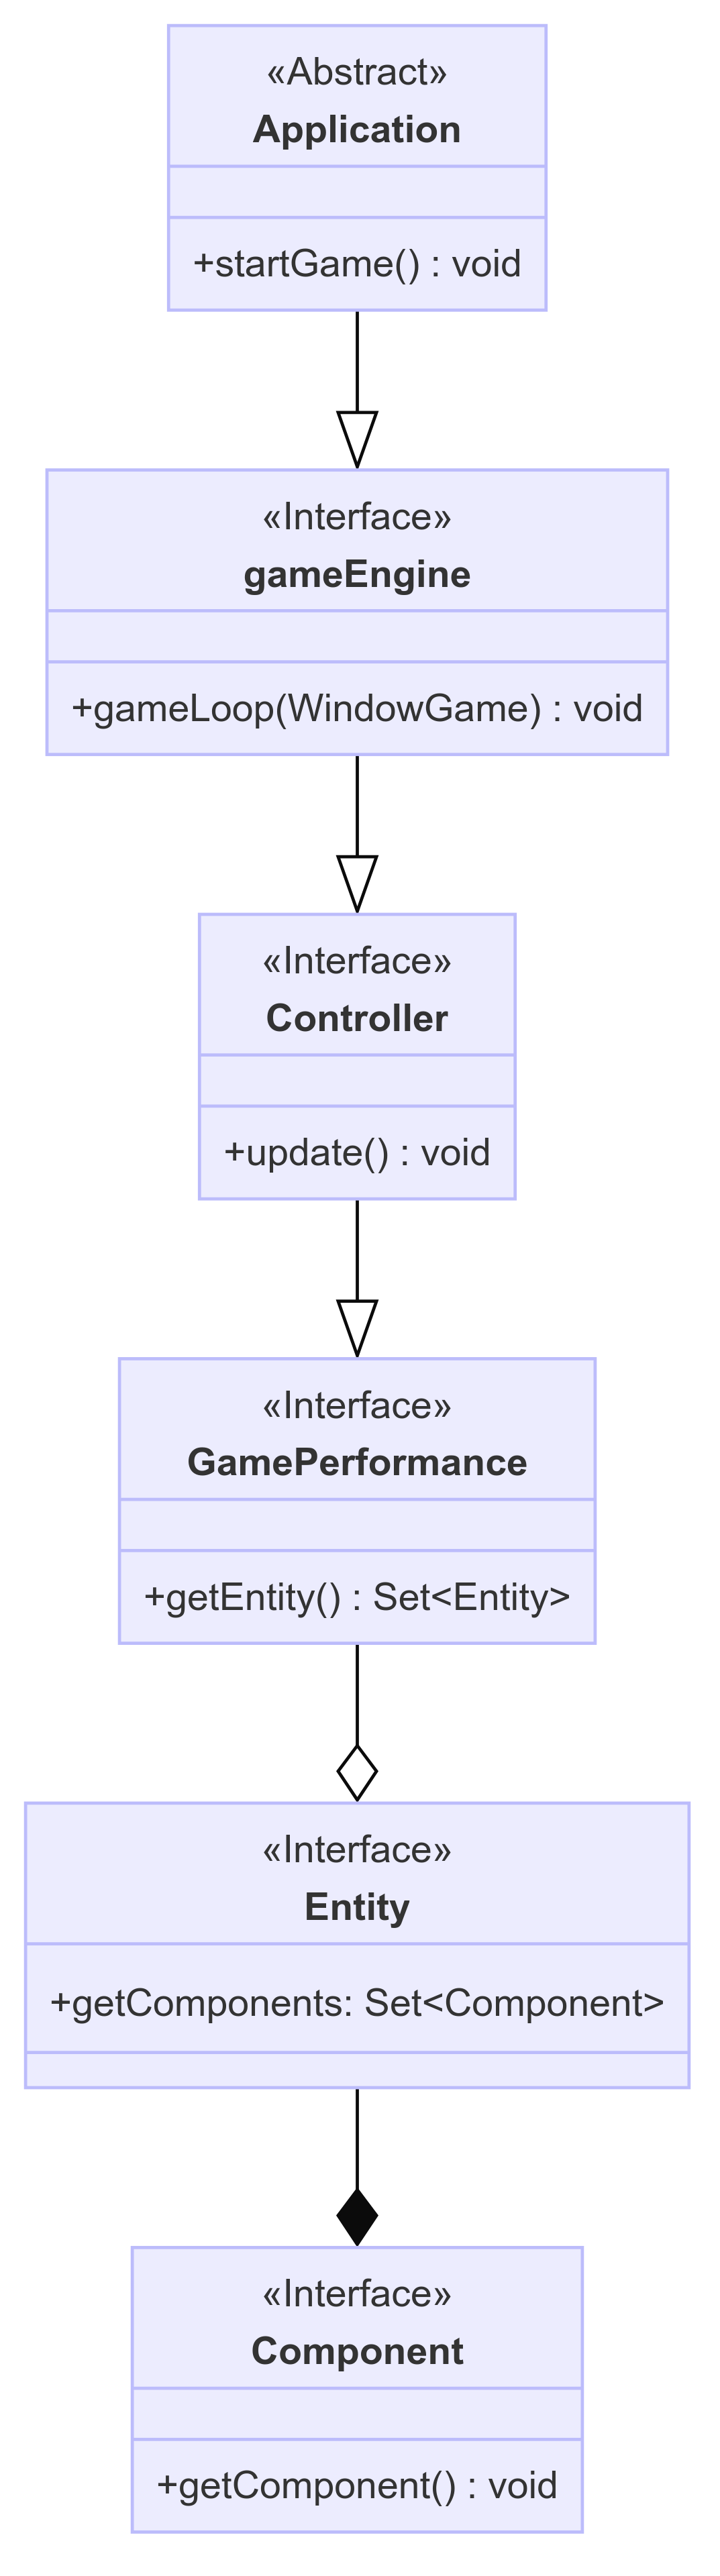
\includegraphics[width=1\textwidth]{img/analisi.png} 
\centering{}
\caption{Schema UML dell'analisi del problema, con rappresentate le entità principali ed i rapporti fra loro}
\label{img:analisi}
\end{figure}

\chapter{Design}

\section{Architettura}
Per realizzare il progetto abbiamo adottato il pattern architetturale MVC (Model-View-Controller) rispettando il più possibile tale suddivisione. 
Ogni suddivisione gestisce una parte diversa: "model” gestisce la logica e i dati del gioco, “view” gestisce la parte grafica, che in base allo stato di gioco (menu, playing, settings, win, death. . . ) disegnera la corretta finestra, infine “controller” ha il compito di interporsi tra model e view per permetterne la comunicazione. 
Abbiamo inoltre scelto di adottare il pattern ECS (Entity-Component System) per la parte di Model, in particolare ogni oggetto di gioco é un’entita che può essere composta da component, ognuno dei quali descrive uno specifico comportamento. 

\begin{figure}[H]
\centering{}
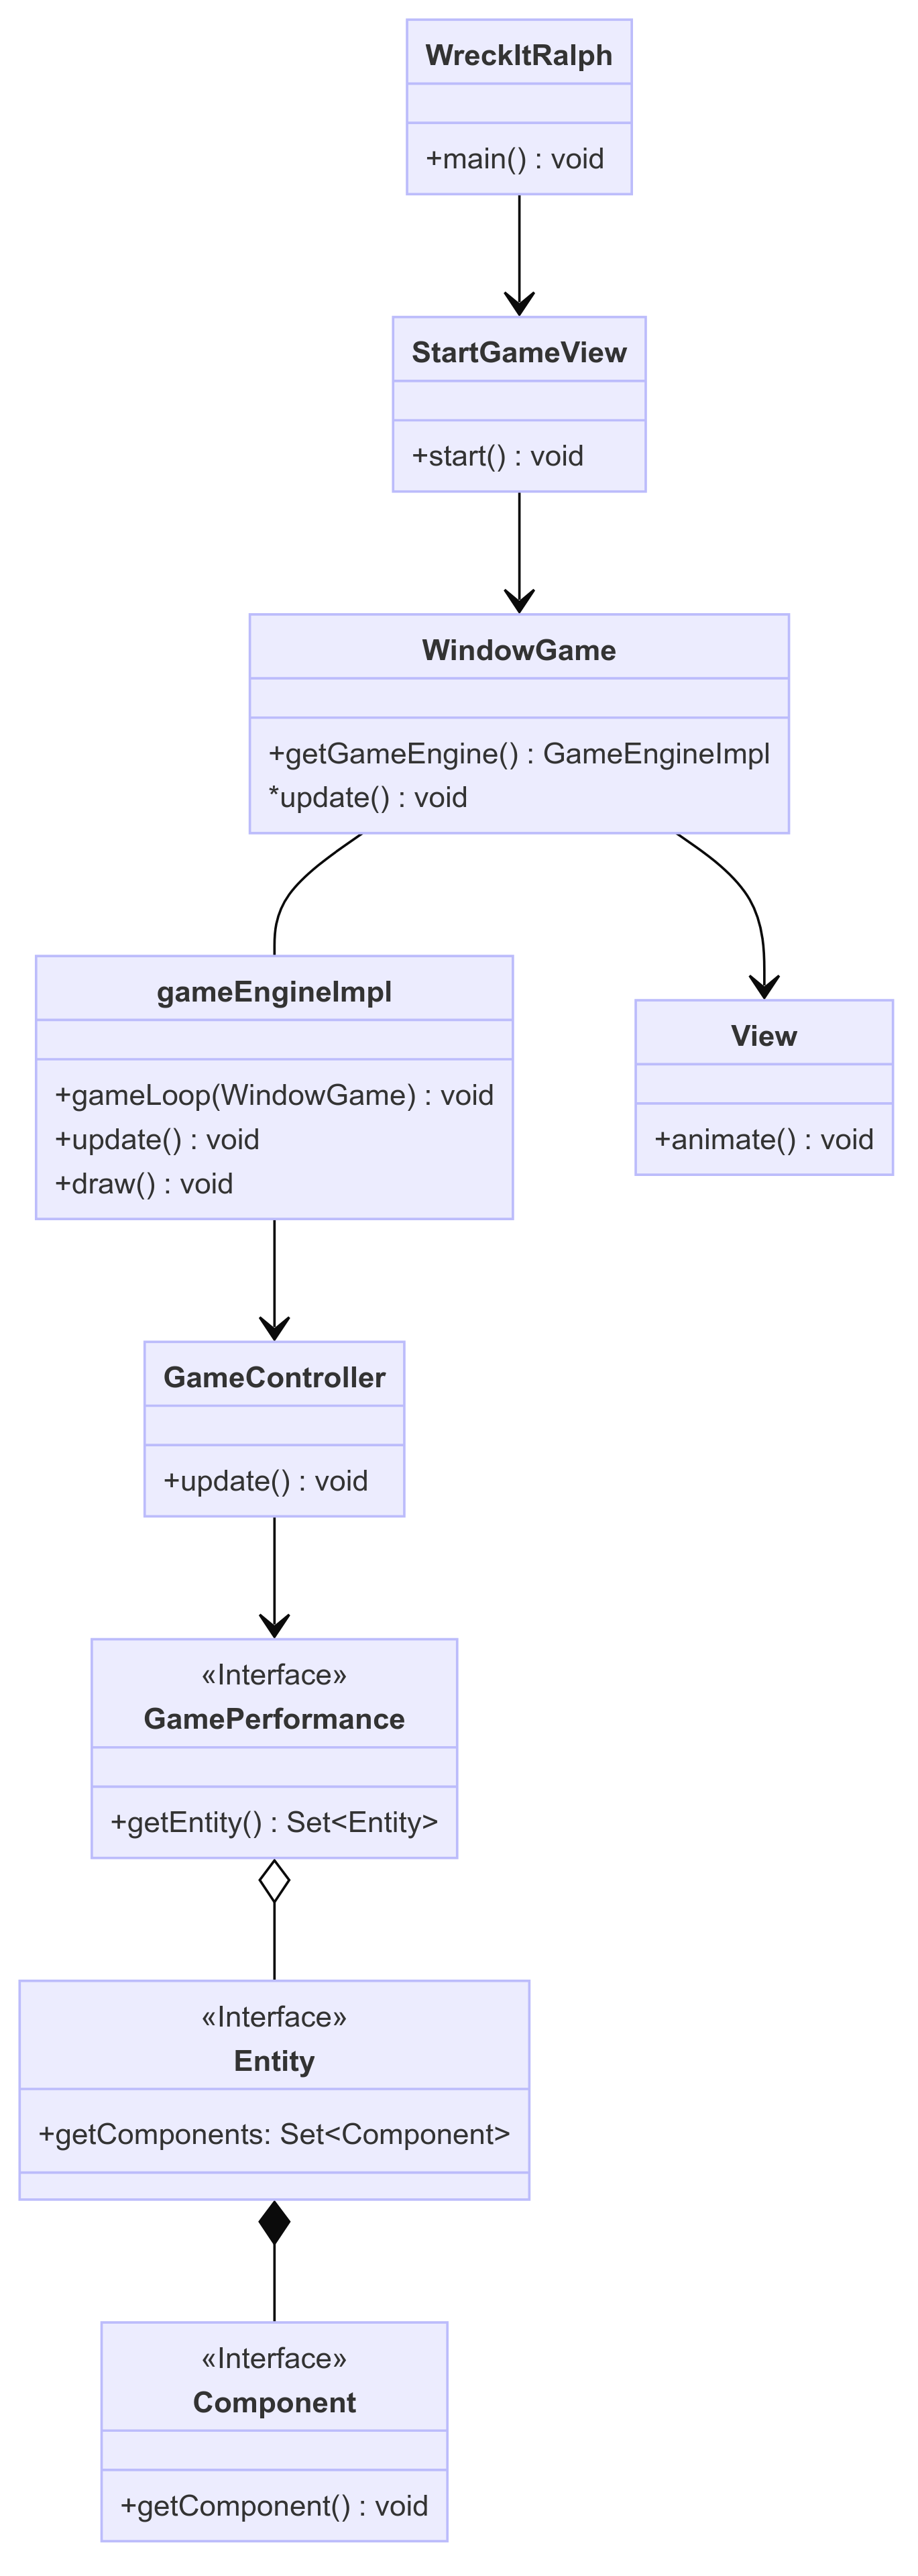
\includegraphics[width=1.25\textwidth]{img/architettura.png}
\caption{Schema UML architetturale di DonkeyKong.}
\label{img:architettura}
\end{figure}

\section{Design dettagliato}
\subsection{Nikolai Zanni}

\subsubsection{Implementazione del menù}

\begin{figure}[H]
\centering{}
\includegraphics[width=\textwidth]{img/menu.png}
\caption{Rappresentazione UML della gestione MVC per il menu.}
\end{figure}

\paragraph{Problema:}
Il gioco possiede un menù iniziale dal quale è possibile avviare una partita, modificare le impostazioni, scegliere un livello o uscire dal gioco.

\paragraph{Soluzione:}
Stati e View già caricati con l'esecuzione del gioco. Quando viene chiamato draw() all’interno della view saranno disegnati tutti gli elementi grafici dell’attuale stato di gioco, per esempio trovandoci nel menu, il background eccetera. Quando si ottiene un input che sia da mouse o da tastiera, in questo caso per ora solo il primo (il secondo `e messo in vista di implementazioni future) in base al bottone che viene premuto sar`a notificato al controller uno stato da applicare che sar`a passato al model e poi eseguito. In caso il bottone premuto fosse quello che poi ci porta all’inizio di una partita allora sar`a settato di default il livello uno, quello considerato iniziale, tramite le chiamate setLevel() e avviata la partita tramite startGame().

\subsubsection{Scelta dei livelli}

\begin{figure}[H]
\centering{}
\includegraphics[width=\textwidth]{img/levels.png}
\caption{Rappresentazione UML della gestione della scelta dei livelli.}
\end{figure}

\paragraph{Problema:}
Nel menu di scelta dei livelli è possibile tornare al menu oppure scegliere un livello.

\paragraph{Soluzione:}
Come per il Menu, in questa schermata `e possibile iniziare una partita, la differenza risiede nel fatto che sono presenti quattro pulsanti diversi (escluso quello per tornare al menu che `e uguale in tutte le schermate) che ci permettono di iniziare quattro livelli unici. Quando la view riceve un punto premuto dal mouse, se `e stato premuto un pulsante che fa iniziare la partita, viene controllato quale deve essere impostato e inviato al menu. che tramite handleChoosenLevel(CurrentLevel level) lo passa al model che esegue il setLevel(CurrentLevel level). Notiamo in questo caso che a differenza del menu, i metodi sopra citati lavorano con un parametro CurrentLevel (enum per la gestione dei livelli) dato che abbiamo la scelta; ovviamente viene anche chiamato il metodo startGame().

\subsubsection{Gestione del settings}

\begin{figure}[H]
\centering{}
\includegraphics[width=\textwidth]{img/settings.png}
\caption{Rappresentazione UML della gestione del settings.}
\end{figure}

\paragraph{Problema:}
Quando ci ritroviamo nella schermata delle impostazioni `e possibile tornare al menu, modificare l’audio disattivandolo o attivandolo e cambiare musica di sottofondo.

\paragraph{Soluzione:}
Prettamente simile a quella del Menu, ma con differenza che da questa schermata non ci `e permesso avviare una partita; semplicemente quando la view ricever`a un punto premuto dal mouse, se sar`a sopra un buttone verr`a applicato lo stato di riferimento, in caso della pressione dei pulsante di gestione audio, sar`a effettuata l’azione corretta.

\subsubsection{Gestione della schermata finale e di pausa}

\begin{figure}[H]
\centering{}
\includegraphics[width=\textwidth]{img/end_stop.png}
\caption{Rappresentazione UML della schermata finale e pausa.}
\end{figure}

\paragraph{Problema:}
Nella schermata di pausa `e possibile ritornare al gioco menu, mentre in quella di fine, ovvero vittoria o sconfitta `e possibile ricominciare il livello da capo. In entrambe `e possibile tornare al menu.

\paragraph{Soluzione:}
Il pulsante per il Menu funziona come per le altre schermate, in questo caso durante lo sviluppo mi sono reso conto che le schermate erano praticamente tutte identiche, di conseguenza ho deciso di controllare lo stato in cui mi trovo all’interno del draw() in modo da visualizzare solo gli elementi grafici corrispondenti. Il metodo startGame() viene utilizzato quando ci si trova nella schermata di fine, mentre in quella di pausa si procede semplicemente riprendendo la partita in corso. Quando ci si trova nella schermata di pausa sono presenti le stesse impostazioni audio della schermata Settings, semplicmente in questa schermata potremo scegliere tra due musiche di gioco diverse da quelle di menù.



\subsection{Cornacchia Enrico}

\subsubsection{Gestione delle entità}

\begin{figure}[H]
\centering{}
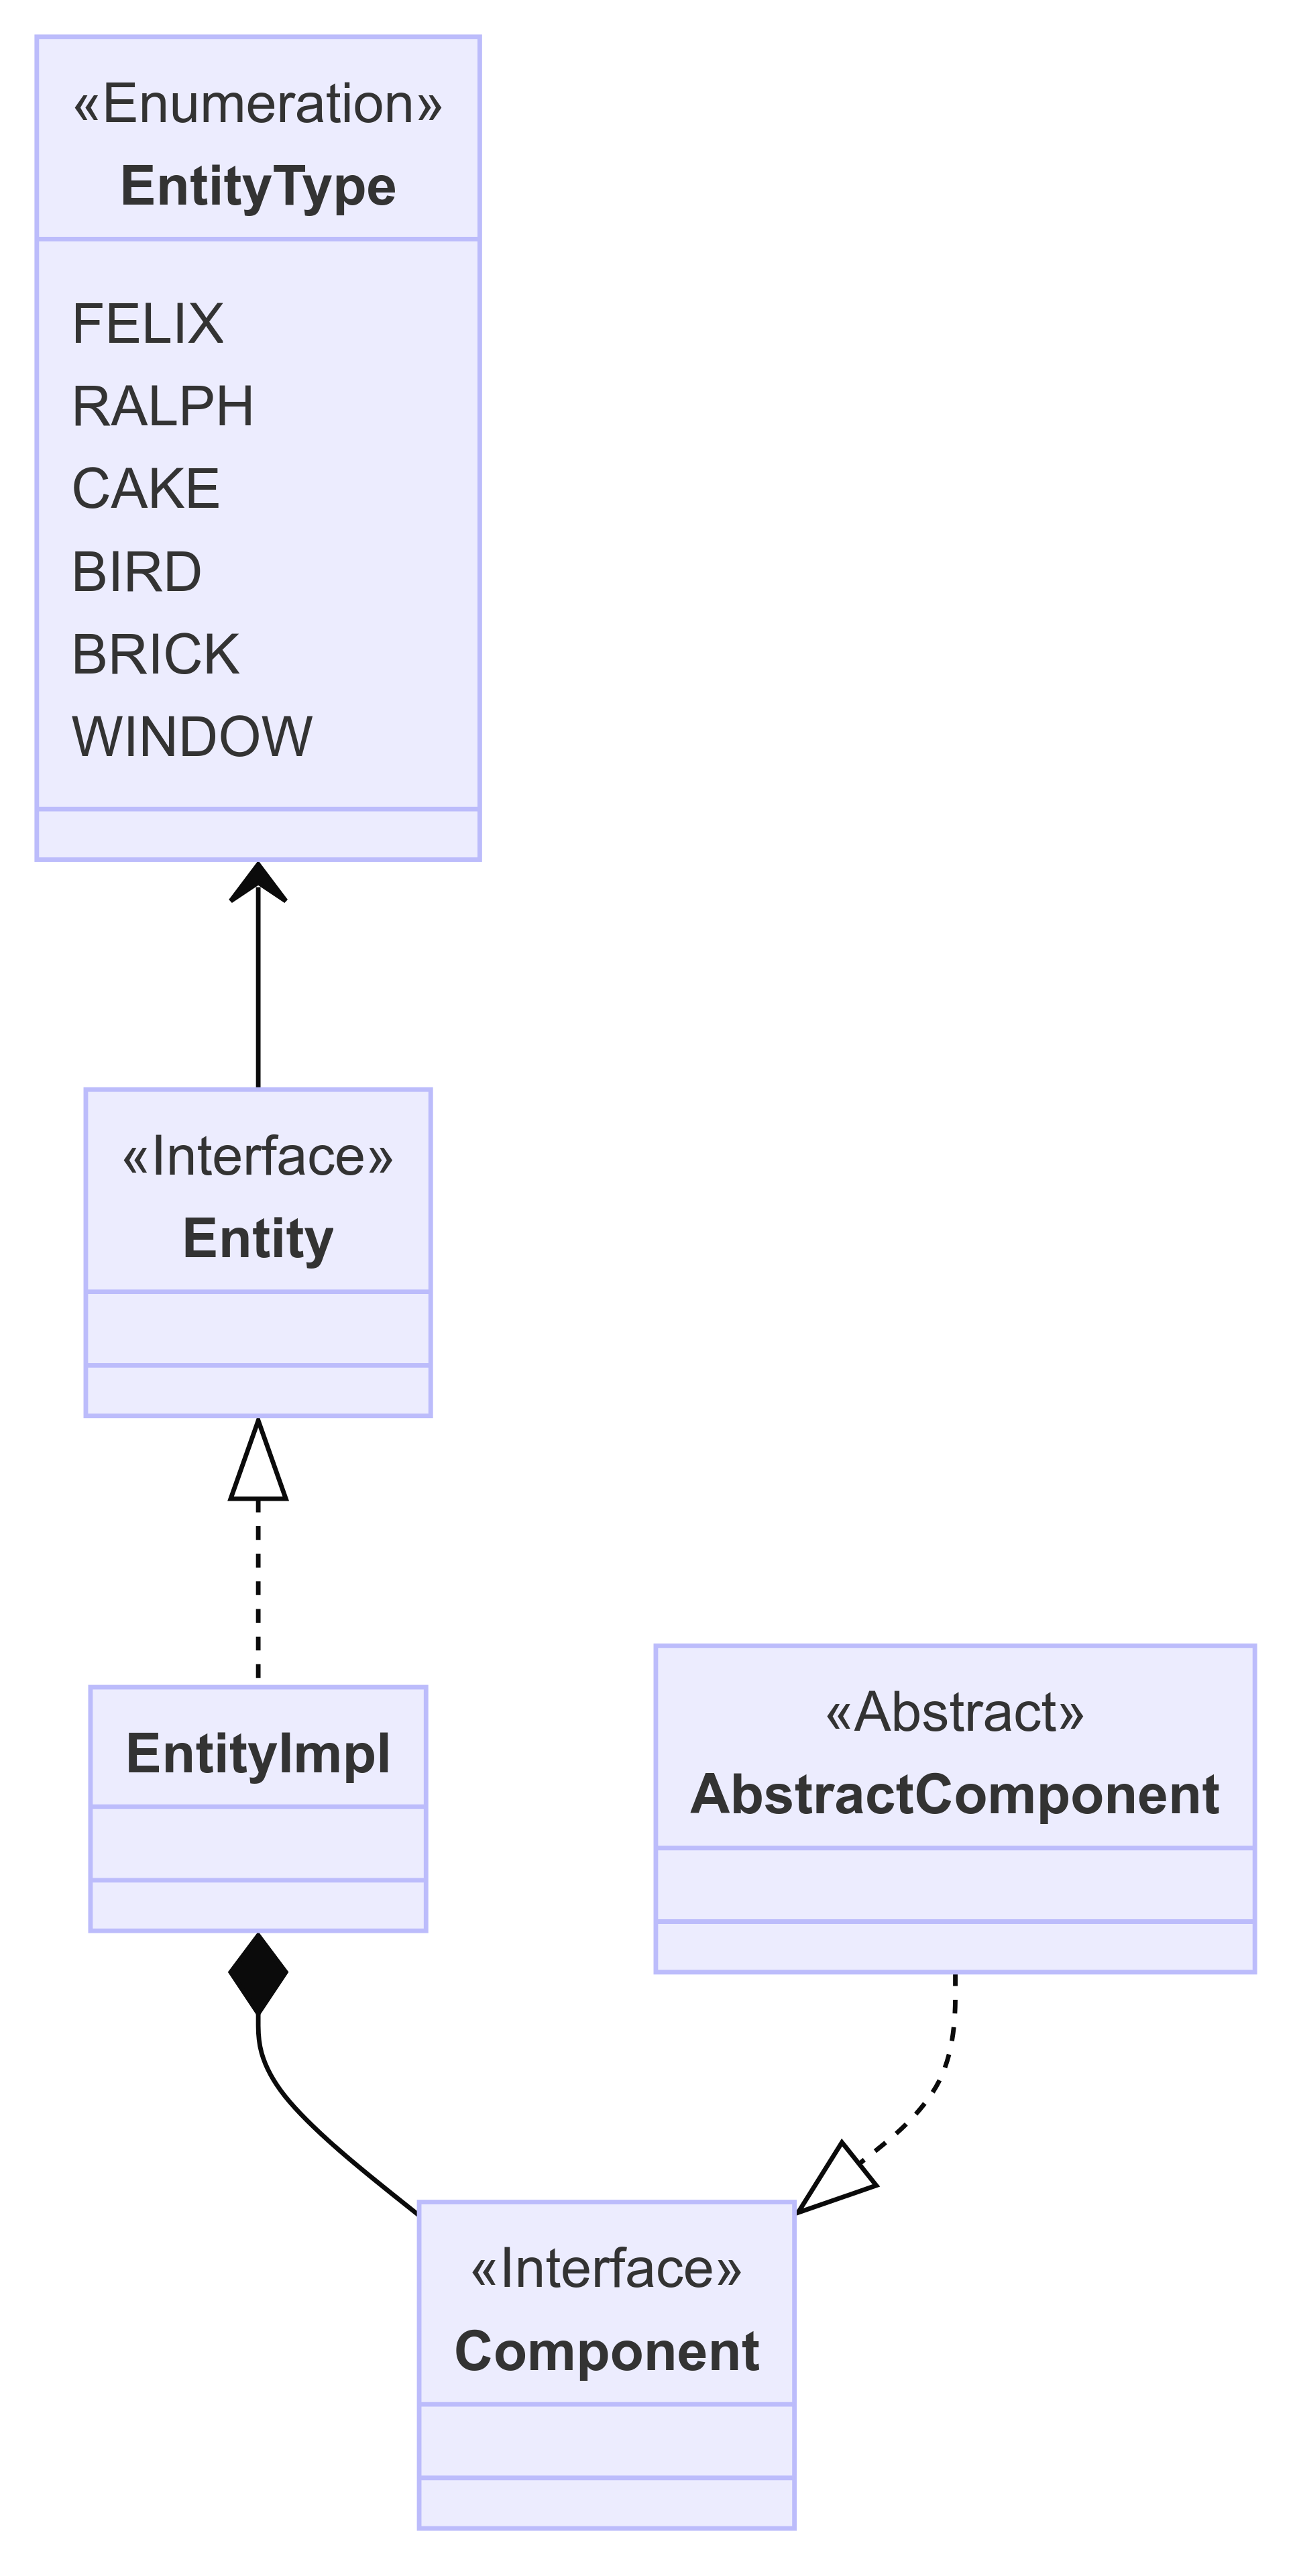
\includegraphics[width=\textwidth]{img/entities.png}
\caption{Rappresentazione UML dell'implementazione delle entità.}
\end{figure}

\paragraph{Problema:}
Le entità sono una parte fondamentale se non il cuore del gioco, di conseguenza ne `e opportuna una gestione ottimale, soprattutto considerando il possibile e non raro caso in cui diverse entit`a possano avere un comportamento uguale o simile.

\paragraph{Soluzione:}
Per ovviare al problema della ripetizione di codice data da possibili comportamenti simili o uguali, `e stato utilizzato il Component Pattern. Ogni entit`a `e un egual guscio vuoto, al quale possiamo aggiungere component specifici o meno durante la creazione. Questo permette un’efficace gestione delle implementazioni delle entit`a rendendo modifiche, ulteriori implementazioni ed estensioni facilmente apportabili e riutilizzabili.

\subsubsection{Gestione della creazione delle entità}

\begin{figure}[H]
\centering{}
\includegraphics[width=\textwidth]{img/create_entities.png}
\caption{Rappresentazione UML della gestione della creazione delle entità.}
\end{figure}

\paragraph{Problema:}
Sia all’inizio del gioco che durante, `e necessario creare diverse entità con diversi component in base ai comportamenti.

\paragraph{Soluzione:}
Il Factory Pattern ci fornisce un metodo centralizzato per la creazione di nuove istanze di entit`a, diverse e con component diversi in modo semplice e veloce. Questo ci offre diversi vantaggi, separa la logica di creazione delle entit`a dal resto dell’applicazione, rendendo il codice pi`u modulare e in caso futuro, di modificare la creazione, i parametri o i component di una o pi`u entit`a molto pi`u semplicemente. La factory pu`o prendere in ingresso parametri per la creazione di queste entit`a come per esempio la posizione.

\subsubsection{Gestione dei power ups}

\begin{figure}[H]
\centering{}
\includegraphics[width=\textwidth]{img/power_ups.png}
\caption{Rappresentazione UML della gestione dei power ups.}
\end{figure}

\paragraph{Problema:}
Il giocatore deve poter usufruire di eventuali powerup sparsi per la mappa i quali forniscono potenziamenti. Anche i barili possono avere powerup, come il danno doppio.

\paragraph{Soluzione:}
Ho deciso di creare un component per ogni powerup, in modo da ottenere una gestione semplice, efficace e facilmente estendibile, ognuno di essi eredita update() da AbstractComponent sfruttando il Template MethodPattern. Ognuno di essi ha un metodo set e get: tramite il primo impostiamo lo stato del power up, il secondo ci ritorna lo stato stesso. Si nota che tra i power up presenti c’`e anche SlowComponent, il quale per`o non viene mai effettivamente utilizzato, questo perch`e `e stato inserito in vista futura. In ogni caso per poterlo utilizzare basterebbe semplicemente aggiungerlo ad un entità.




\subsection{Golesano Giulia}

\subsubsection{Gestione della schermata di gioco}

\begin{figure}[H]
\centering{}
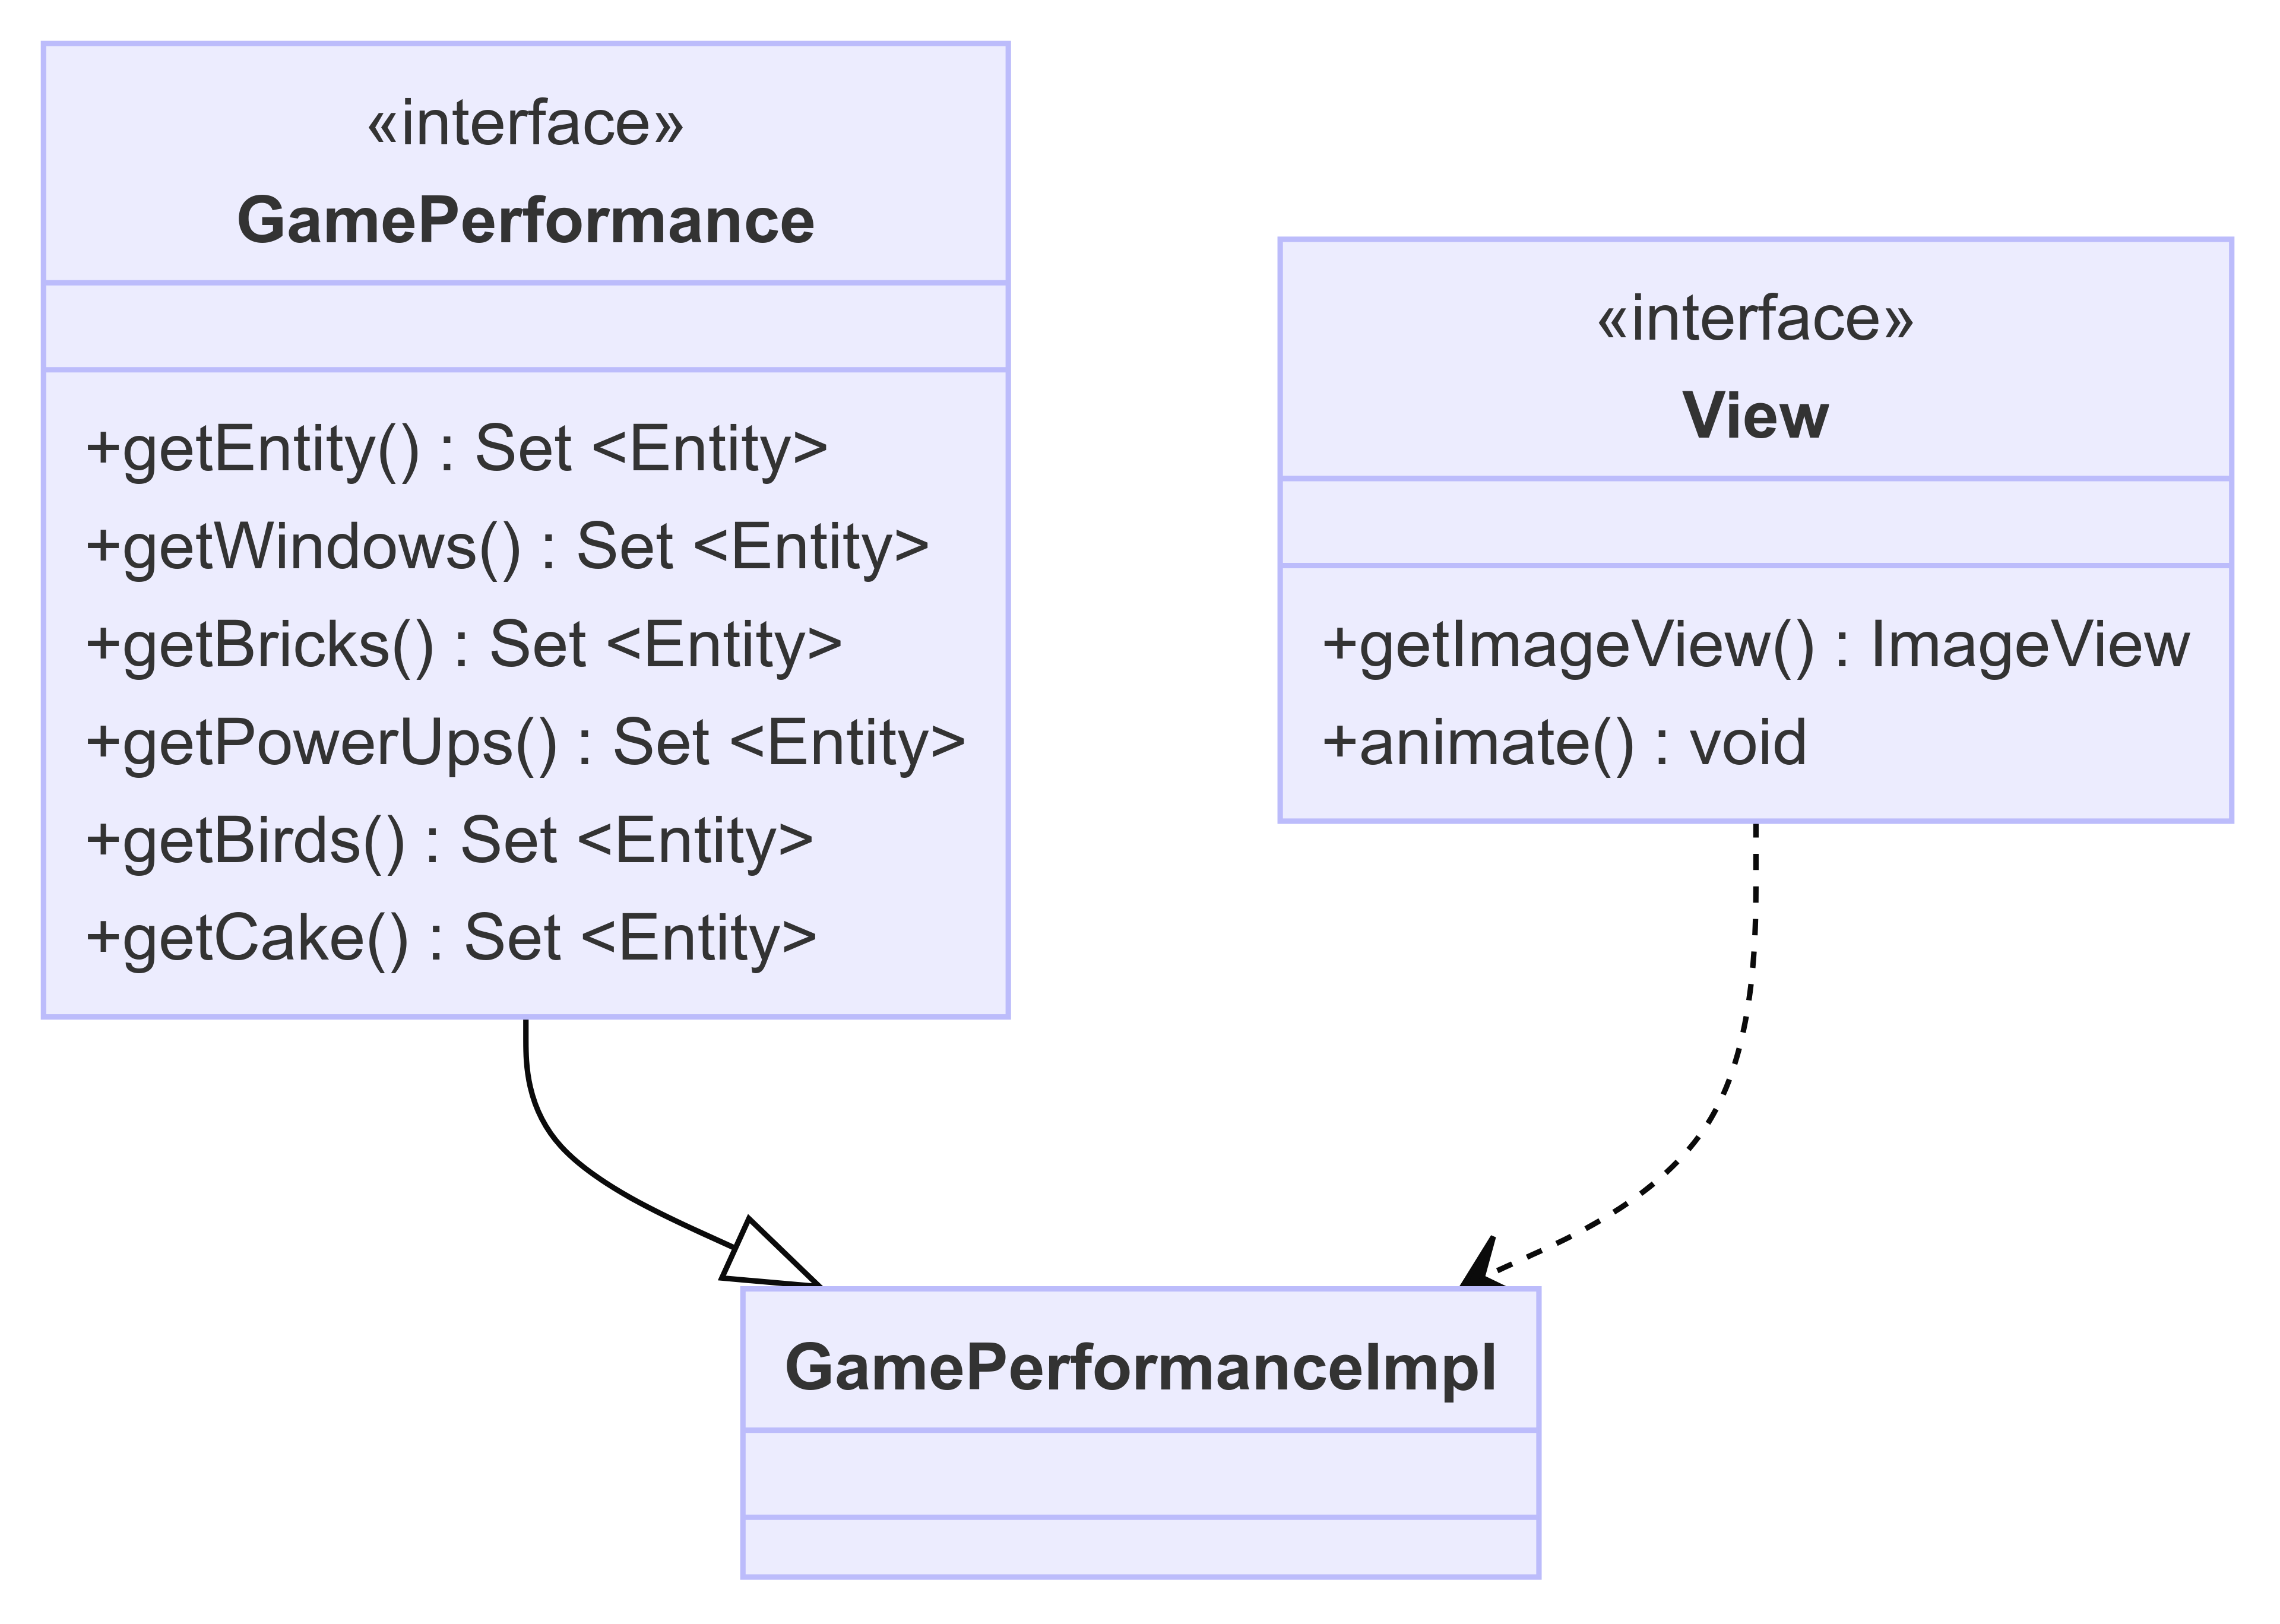
\includegraphics[width=\textwidth]{img/game.png}
\caption{Rappresentazione UML della gestione della schermata di gioco.}
\end{figure}

\paragraph{Problema:}
Gestione della schermata di gioco: delle entità presenti, delle loro posizioni, dei loro possibili movimenti, delle vite, dei punteggi e dei funzionamenti pratici del gioco.

\paragraph{Soluzione:}
Ho creato un'interfaccia GamePerformance che ha lo scopo di gestire tutti i funzionamenti pratici della partita, con relative implementazioni nella classe GamePerformanceImpl.
Per quanto riguarda gli sprites delle entità, i cui indici devono essere aggiornati ciclicamente per realizzare una animazione, già caricate nella cartella Resources; ho creato un'interfaccia View che ha lo scopo di disegnare una view, tramite apposito metodo draw, e gestire gli input da tastiera e da mouse, che ne determinano i cambiamenti, tramite apposito metodo update.
Tale metodo richiede al GameController di aggiornare gli indici .
La view quando viene creata instanzia un oggetto LevelImpl che crea il livello da giocare, `e stato inserito nella view dato che utilizzo librerie grafiche per caricare la mappa, mi avvalgo di una immagine pixel per pixel dove in base all’indice RGB, nel nostro caso rosso, ci permette di ottenere la posizione e il tipo di blocco presente. Tramite getLevelMap() si restituiscono solo i valori interi sia delle posizioni che dei blocchi, per poterli poi passare al gameplay al momento della creazione e inizializzare correttamente le entit`a del livello (per esempio blocco).

\subsubsection{Gestione listener generici di input da tastiera e mouse}

\begin{figure}[H]
\centering{}
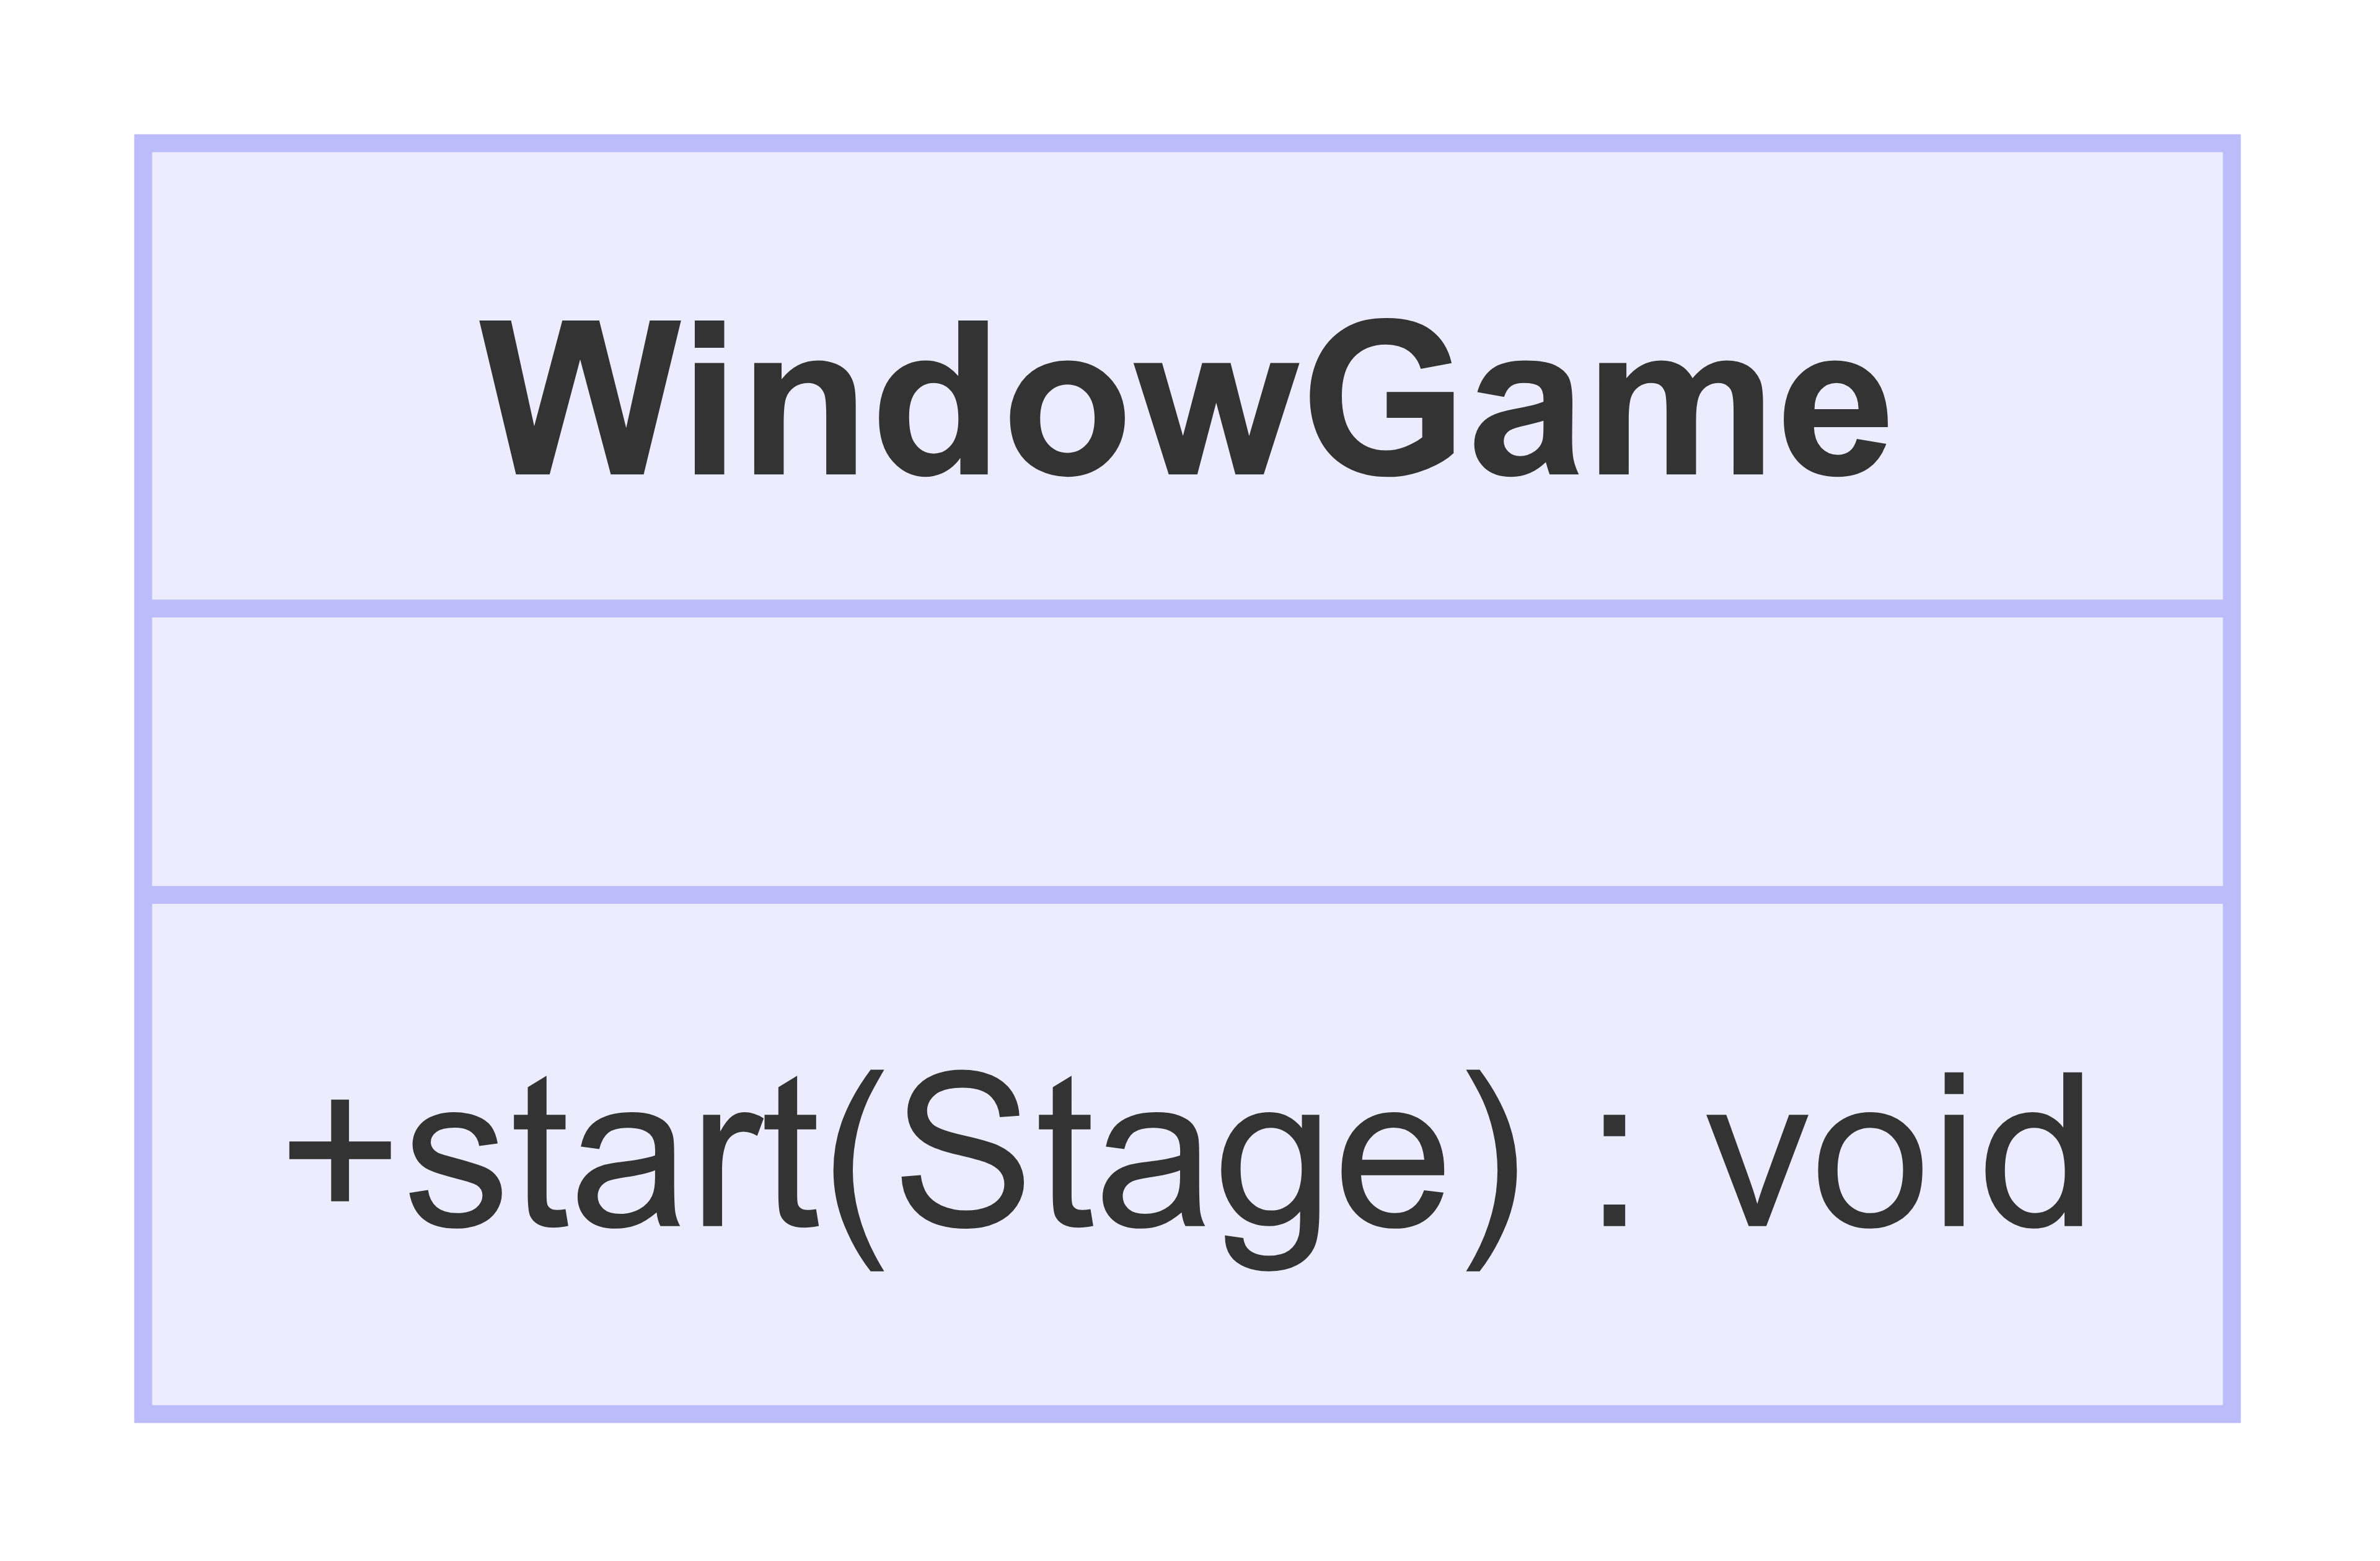
\includegraphics[width=\textwidth]{img/input.png}
\caption{Rappresentazione UML della gestione listener generici di input da tastiera e mouse.}
\end{figure}

\paragraph{Problema:}
Per giocare è necessario far muovere il giocatore sulla schermata di gioco, così da poter vincere e superare i livelli.

\paragraph{Soluzione:}
Rispettando il più possibile il pattern architetturale MVC, ho gestito gli input da tastiera tramite un apposito EventHandler nel pannello di View con maggior priorità. Il KeyCode registrato dall'evento l'ho poi passato alla classe principale di Controller che, a sua volta, lo ha delegato al Controller specifico del personaggio in grado di muoversi, e ha fatto si che la classe generale di Model registrasse il dato nella sua lista di input.

\subsubsection{Creazione delle finestre}

\begin{figure}[H]
\centering{}
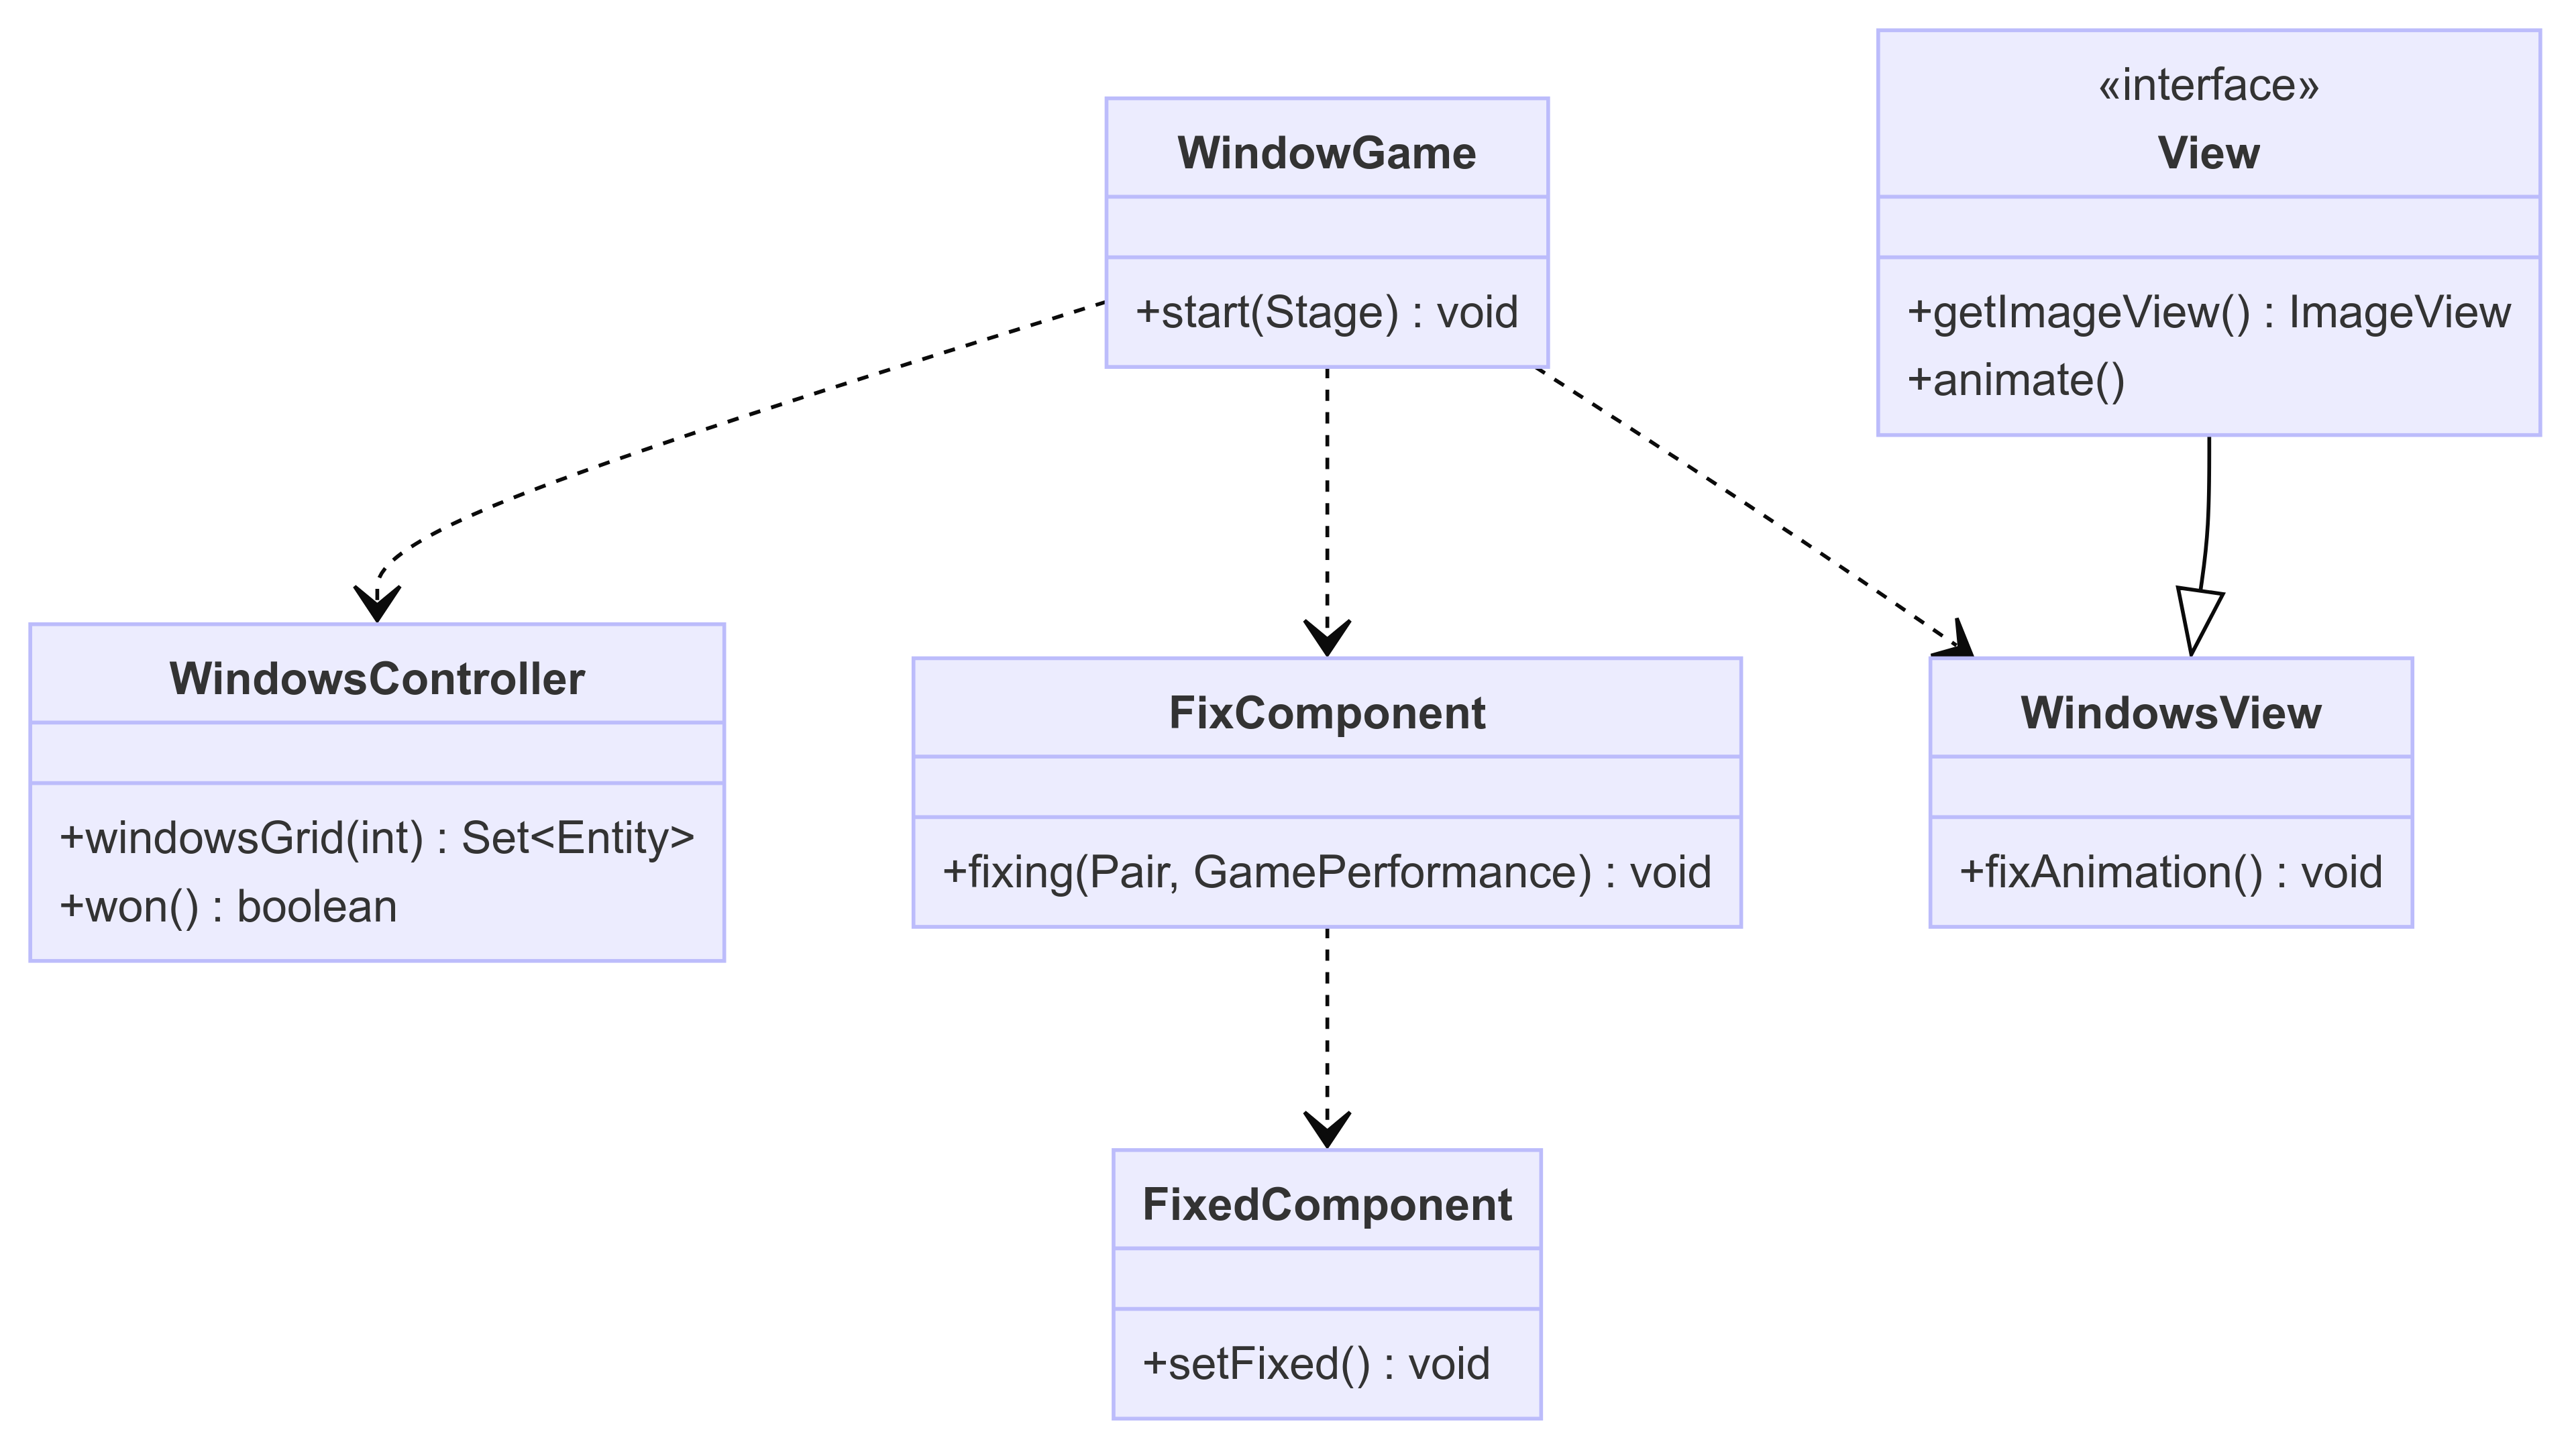
\includegraphics[width=\textwidth]{img/windows.png}
\caption{Rappresentazione UML della gestione delle collisioni.}
\end{figure}

\paragraph{Problema:}
Il gioco obbligatoriamente deve gestire le varie collisioni tra entit`a o con i bordi del livello.

\paragraph{Soluzione:}
Studiando il problema mi sono reso conto che un’ottima soluzione per il controllo delle collisioni fosse predisporre ogni Entit`a di una hitbox, un oggetto Rectangle che possiede un metodo che mi permette di sapere quando due di essi collidono. Utilizzo il Template Method Pattern, eredito update() da AbstractComponent, che ad ogni richiamo controlla se la relativa entit`a `e in collisione con un’altra gestendone le conseguenze.






\subsection{Rinchiuso Giovanni}

\subsubsection{Gestione del GameEngine}

\begin{figure}[H]
\centering{}
\includegraphics[width=\textwidth]{img/gameloop.jpg}
\caption{Rappresentazione UML del game engine.}
\end{figure}

\paragraph{Problema} Il gioco deve essere in grado di permettere un gameplay fluido senza lag, aggiornando ciclicamente la grafica (view) e la logica di gioco (model) in contemporanea.

\paragraph{Soluzione} Ho deciso di scorporare la gestione del game loop dal controller principale (Application) implementando un’interfaccia GameEngine, al fine di evitare la condivisione di codice sensibile e garantire una maggiore indipendenza, permettendo così di estendere anche in altre classi, in caso di bisogno, il motore del gioco. Il GameEngine viene fatto partire all’avvio dell’applicazione dal controller, richiamando il metodo mainLoop(), nucleo vero e proprio del game che gestisce il ciclo e fa in modo che non si verifichino perdite di frame. Tuttavia, durante lo sviluppo, mi son reso conto che è necessario aggiornare la parte di model e gestione delle varie entità solo nel caso in cui si stia effettivamente giocando; per questa ragione il suddetto metodo prevede che nel caso in cui ci si trovi nel menù iniziale, di pausa, o finale (vittoria o sconfitta), venga aggiornata solo la grafica e non la logica di gioco, risparmiando memoria e processi inutili.

\subsubsection{Gestione di inizio gioco}

\begin{figure}[H]
\centering{}
\includegraphics[width=\textwidth]{img/game_start.jpg}
\caption{Rappresentazione UML della logica di inizio gioco.}
\end{figure}

\paragraph{Problema} Avviare una partita in maniera totalmente indipendente ed efficace in qualunque momento e stato dell’applicazione

\paragraph{Soluzione} Per permettere che una nuova partita possa essere sempre iniziata quando viene cliccato il tasto “Play”, ho implementato nel controller principale Application un metodo startGame(). Esso va a creare un nuovo GameController, che si occupa a sua volta di creare un nuovo Gameplay. Attraverso il metodo initializeGame() di quest’ultimo, verranno poi inizializzate tutte le istanze necessarie affinchè si possa giocare una partita.

\subsubsection{Gestione di fine gioco}

\begin{figure}[H]
\centering{}
\includegraphics[width=\textwidth]{img/gameplay.jpg}
\caption{Rappresentazione UML della logica di fine gioco.}
\end{figure}

\paragraph{Problema} Controllare che il giocatore abbia perso o vinto una partita.

\paragraph{Soluzione} Per fare in modo che fosse verificata la condizione di vittoria e sconfitta e fosse aggiornato il Gamestate, ho utilizzato un metodo update() all’interno del controller di gioco, che viene eseguito ad ogni ciclo. Questo verifica la condizione di vittoria o sconfitta; se la partita è terminata, aggiorna solamente la grafica senza aggiornare le entità. Per fare ciò, richiama i metodi del gameplay checkIsOver(), isOver(), e setIsWin(). I primi due verificano che esista ancora un player nella lista delle entità di gioco: nel caso non esistesse, cambia il Gamestate in Death e fermano il timer di gioco. Il terzo, è un metodo che viene richiamato all’interno delle Collision quando l’entità del player va a collidere con la principessa, e setta il Gamestate a Win (fermando anch’esso il timer di gioco).

\subsubsection{Gestione dei mattoni}

\begin{figure}[H]
\centering{}
\includegraphics[width=\textwidth]{img/throw.jpg}
\caption{Rappresentazione UML della logica di spawn dei barili.}
\end{figure}

\paragraph{Problema} Gestione dello spawn dei mattoni durante la partita.

\paragraph{Soluzione} Per gestire la generazione delle entità mattoni durante la partita da parte del nemico (Donkey Kong), ho implementato un Component da associare esso, sfruttando così il Template Method Pattern, ereditando update() da AbstractComponent. Questo verifica se DK si trova in uno stato di congelamento per via di un powerup, e quindi se non deve generare barili, o se al contrario gli è concesso lanciare gli ostacoli.

\chapter{Sviluppo}
\section{Testing automatizzato}
\section{Metodologie di lavoro}
\section{Note di sviluppo}

\chapter{Guida Utente}


